\documentclass[xcolor=table]{beamer}
\usepackage{graphicx}
\usepackage[spanish]{babel} % para escribir en espanol
\usepackage[utf8]{inputenc}
\usepackage{wrapfig}

\graphicspath{ {imagenes/} }

\usetheme{Madrid}

\title{Aplicaciones del análisis multivariante con R}
\subtitle{Estadística Multivariante - Universidad de Granada}

\author{Miguel Lentisco Ballesteros \\ Francisco Javier Sáez Maldonado \\Daniel Pozo Escalona \\Antonio Martín Ruiz \\ Laura Gómez Garrido}

\AtBeginSection[]
{
  \begin{frame}<beamer>{}
    \tableofcontents[currentsection,currentsubsection]
  \end{frame}
}

\begin{document}
\begin{frame}
\titlepage
\end{frame}
\begin{frame}{Contenido}
  \tableofcontents
  % You might wish to add the option [pausesections]
\end{frame}
\section{Introducción: R}

\begin{frame}{¿Qué es R?}

R es un entorno y lenguaje de programación enfocados a la computación estadística y de gráficos. Surge como una reimplementación libre del lenguaje y entorno S. Proporciona una amplia variedad de funcionalidades estadísticas y gráficas y es altamente extensible.
\newline
\newline
R está disponible como software libre bajo los términos de la GNU General Public License de la Free Software Foundation en forma de código fuente. Puede ser compilado y ejecutado en una gran cantidad de plataformas UNIX, Windows y MacOs.

\end{frame}

\begin{frame}{Entornos de desarrollo para R}
\end{frame}

\begin{frame}{Principales librerías}

\end{frame}

\begin{frame}{Algunas aplicaciones de R}
\end{frame}

\section{R en el análisis multivariante}
\begin{frame}{Nuestro dataset}

\begin{table}[]
\resizebox{10cm}{!}{
\begin{tabular}{|
>{\columncolor[HTML]{979CD8}}l |l|
>{\columncolor[HTML]{979CD8}}l |l|}
\hline
\textbf{Característica del data set}      & Multivariante   & \textbf{Nº de Instancias} & 178        \\ \hline
\textbf{Características de los atributos} & Enteros, Reales & \textbf{Nº de Atributos}  & 13         \\ \hline
\textbf{Área}                             & Física          & \textbf{Donado}           & 01/07/1991 \\ \hline
\end{tabular}
}
\end{table}
\begin{wrapfigure}{r}{0.25\textwidth}
\centering
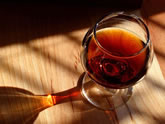
\includegraphics[width=0.25\textwidth]{vino.jpg}
\end{wrapfigure}
{Fuente: Machine Learning Repository\\
Propietarios Originales: }\begin{quote}\scriptsize Forina, M. et al, PARVUS -\\
An Extendible Package for Data Exploration, Classification \\and Correlation.\\
Institute of Pharmaceutical and Food Analysis and Technologies, \\Via Brigata Salerno,
16147 Genoa, Italy.\end{quote}
\end{frame}
\subsection{Distribución Normal Multivariante}
\begin{frame}{Media Muestral}
\begin{verbatim}

Escribes tu código aquí­

\end{verbatim}
\end{frame}

\section{Para ampliar}
\begin{frame}{Para ampliar}
\textit{Computing Machinery and Intelligence} Alan Turing (1950)
\newline
\newline
\textit{Artifficial Intelligence: A Modern Aproach} Stuart J. Russell y Peter Norvig
\newline
\newline
\textit{Concrete Problems in AI Safety} Dario Amodei, Crhis Olah, Jacob Steinahrdt, Paul Christiano, John Schulman, Dan Mané
\newline
\newline
\textit{The Malicious Use of Artificial Intelligence: Forecasting, Prevention, and Mitigation} Miles Brundage, Shahar Avin et al.
\end{frame}
\end{document}
